\begin{pastexam}[label={px:nccu-114-dsa-16}]{政大資科所 114 學年度 第 16 題}
（設計；20 分）

(20\%) Six Degrees of Separation is the theory that any person on the planet can be connected to
any other person on the planet through a chain of acquaintances that has no more than five
intermediaries on average. For example, in Figure 1, the degree of separation between Gia and
Felix is five. They can be connected by at least four intermediaries. The average degree of
separation in this social network is about 2.1. Given a dense social network of $n$ persons,
design a dynamic programming algorithm to compute the average degree of separation in this social
network.\\
(1) (10\%) Give the algorithm in pseudo code clearly.\\
(2) (5\%) Give the recurrence relation.\\
(3) (5\%) Analyze the time complexity of your algorithm.
\begin{center}
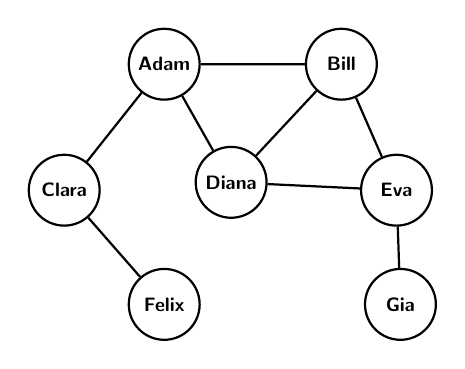
\begin{tikzpicture}[x=1cm,y=1cm,
  p/.style={circle,draw,thick,inner sep=0pt,minimum size=9mm,font=\sffamily\bfseries\scriptsize},
  every path/.style={thick}]
  \node[p] (Adam) at (2.05,-1.3) {Adam};
  \node[p] (Bill) at (4.3,-1.3) {Bill};
  \node[p] (Clara) at (0.78,-2.9) {Clara};
  \node[p] (Diana) at (2.9,-2.8) {Diana};
  \node[p] (Eva) at (5.0,-2.9) {Eva};
  \node[p] (Felix) at (2.05,-4.35) {Felix};
  \node[p] (Gia) at (5.05,-4.35) {Gia};
  \draw (Adam)--(Bill) (Adam)--(Clara) (Adam)--(Diana) (Bill)--(Diana) (Bill)--(Eva)
        (Diana)--(Eva) (Clara)--(Felix) (Eva)--(Gia);
\end{tikzpicture}\\
Figure 1
\end{center}
\end{pastexam}

\begin{pastsoln}
社交網路看成無向、不加權的圖：每個人是一個頂點，兩人認識就連一條邊。 兩人之間的 degree of
separation 是他們之間最短路徑的\textbf{邊數}（Gia 到 Felix 是 Gia--Eva--Bill--Adam--Clara--Felix，
$5$ 條邊、中間 $4$ 個人）。 平均值就是所有 $\binom{n}{2}$ 對人的最短距離的平均。 所以要求的是全點對
最短路徑，題目指定動態規劃，用 Floyd--Warshall 演算法（資結書第~25.6~節、虛擬碼~25.8）。 網路是
稠密的，用鄰接矩陣存。

不連通的兩個人之間沒有距離。 下面的做法只平均「有路相通」的那些對；如果要求整張圖連通，遇到
$\infty$ 就回報「無法連結」也可以，作答時寫清楚採用哪一種。

\textbf{(2) 遞迴式}。 人編號 $1$ 到 $n$。 令 $d^{(k)}_{ij}$ 是「從 $i$ 到 $j$、中間經過的人只能從
$\{1, 2, \ldots, k\}$ 裡挑」的最短路徑邊數（沒有這樣的路徑時是 $\infty$）。
\[
d^{(0)}_{ij} =
\begin{cases}
0 & i = j, \\
1 & i \ne j \text{ 且 } i, j \text{ 認識}, \\
\infty & \text{其他},
\end{cases}
\qquad
d^{(k)}_{ij} = \min\bigl(d^{(k-1)}_{ij},\ d^{(k-1)}_{ik} + d^{(k-1)}_{kj}\bigr) \quad (1 \le k \le n).
\]
理由：中間點限制在 $\{1, \ldots, k\}$ 的最短路徑，要嘛不經過 $k$，長度是 $d^{(k-1)}_{ij}$；要嘛
經過 $k$ 恰好一次（最短路徑不會重複經過同一點），$k$ 把它切成 $i \leadsto k$ 和 $k \leadsto j$ 兩段，
兩段的中間點都只在 $\{1, \ldots, k - 1\}$ 裡，而且各自都必須是最短的（最佳子結構），長度是
$d^{(k-1)}_{ik} + d^{(k-1)}_{kj}$。 兩者取小的。 $d^{(n)}_{ij}$ 就是真正的最短距離。

\textbf{(1) 虛擬碼}。 $A$ 是 $n \times n$ 的鄰接矩陣，$A[i][j] = 1$ 表示 $i$、$j$ 認識。 和 Floyd--Warshall
一樣，$d^{(k)}$ 可以直接覆蓋在同一個表上（第 $k$ 輪裡 $d_{ik}$、$d_{kj}$ 不會變，因為
$d_{kk} = 0$）。
\begin{pseudo}[unbreakable]{平均分隔度數（Floyd--Warshall）}
\Function{Average-Separation}{$A, n$}
    \For{$i \gets 1$ \To $n$}
        \For{$j \gets 1$ \To $n$}
            \If{$i = j$}
                \State $d[i][j] \gets 0$
            \ElsIf{$A[i][j] = 1$}
                \State $d[i][j] \gets 1$
            \Else
                \State $d[i][j] \gets \infty$
            \EndIf
        \EndFor
    \EndFor
    \For{$k \gets 1$ \To $n$} \Comment{允許經過第 $k$ 個人}
        \For{$i \gets 1$ \To $n$}
            \For{$j \gets 1$ \To $n$}
                \If{$d[i][k] + d[k][j] < d[i][j]$}
                    \State $d[i][j] \gets d[i][k] + d[k][j]$
                \EndIf
            \EndFor
        \EndFor
    \EndFor
    \State $s \gets 0$；$c \gets 0$
    \For{$i \gets 1$ \To $n - 1$}
        \For{$j \gets i + 1$ \To $n$}
            \If{$d[i][j] < \infty$}
                \State $s \gets s + d[i][j]$；$c \gets c + 1$
            \EndIf
        \EndFor
    \EndFor
    \State \Return $s / c$ \Comment{$c = 0$（$n \le 1$ 或沒有任何邊）時沒有定義}
\EndFunction
\end{pseudo}

\textbf{正確性}。 第 10--14 行跑完之後，對 $k$ 歸納可知 $d[i][j] = d^{(k)}_{ij}$，所以最後
$d[i][j]$ 是 $i$ 到 $j$ 的最短距離（資結書第~25.6~節的證明）。 第 15--19 行把每一對人
（$i < j$，每對只算一次）的距離加起來，除以對數，就是平均。

以圖 1 驗證：七個人的最短距離如下表。
\begin{center}
\small
\begin{tabular}{lccccccc}
\toprule
 & Adam & Bill & Clara & Diana & Eva & Felix & Gia \\
\midrule
Adam  & 0 & 1 & 1 & 1 & 2 & 2 & 3 \\
Bill  & 1 & 0 & 2 & 1 & 1 & 3 & 2 \\
Clara & 1 & 2 & 0 & 2 & 3 & 1 & 4 \\
Diana & 1 & 1 & 2 & 0 & 1 & 3 & 2 \\
Eva   & 2 & 1 & 3 & 1 & 0 & 4 & 1 \\
Felix & 2 & 3 & 1 & 3 & 4 & 0 & 5 \\
Gia   & 3 & 2 & 4 & 2 & 1 & 5 & 0 \\
\bottomrule
\end{tabular}
\end{center}
$21$ 對裡距離為 $1, 2, 3, 4, 5$ 的各有 $8, 6, 4, 2, 1$ 對，總和
$8 + 12 + 12 + 8 + 5 = 45$，平均 $45 / 21 \approx 2.14$，和題目說的「about 2.1」一致；Gia 和 Felix
是 $5$。

\textbf{(3) 時間}。 第 2--9 行初始化 $\Theta(n^2)$；第 10--14 行三層迴圈各 $n$ 次，內層 $O(1)$，
$\Theta(n^3)$；第 15--19 行 $\Theta(n^2)$。 總共 $\Theta(n^3)$，空間 $\Theta(n^2)$。

補充：圖不加權，也可以從每個人各做一次 BFS（資結書第~21.3~節）。 用鄰接串列是
$O(n(n + m))$；題目說網路是稠密的，$m = \Theta(n^2)$，也是 $\Theta(n^3)$，和 Floyd--Warshall
同級。 題目指定動態規劃，所以上面用 Floyd--Warshall。
\end{pastsoln}
